\section{$Z$ Transform}
\label{Chap:z_transform}
\begin{frame}[t,allowframebreaks]{Chapter \autoref{Chap:z_transform}}
\tableofcontents[sections= \value{section}]
\end{frame}


\subsection{Complex Exponential Signal}
\begin{frame}[t,allowframebreaks]{Some Preliminary}

\begin{itemize}

\item Before we dive in the definition of $Z$-transform, let's see what is this number called $z$

	\begin{itemize}
	\item This will give us some intuition since we use this number in the definition oft the $Z$-transform
	\end{itemize}

\item $z$ is just a \textcolor{red}{complex number} 

\item We prefer to write in polar form as $z \, = \, r \, e^{j \, \Omega}$

\item If we form a signal called $x[k] \, = \, z^{k}$, it will be a \textcolor{red}{discrete time complex signal}, where using Euler identity we have:

\begin{equation*}
x[k] \, = \, z^{k} \, = \, r^k \, \left[\, \text{cos}(\Omega \, k) \, + \, \text{sin}(\Omega \, k)  \,\right]
\end{equation*}

	\begin{itemize}
	\item $r$ controls the damping of this signal
	
	\item and $\Omega$ controls the frequency
	\end{itemize}

\newpage
\item An example is shown in figure \autoref{fig:z_transform:exp_signal} for $r \, < \, 1$

\begin{figure}[ht]
\centering
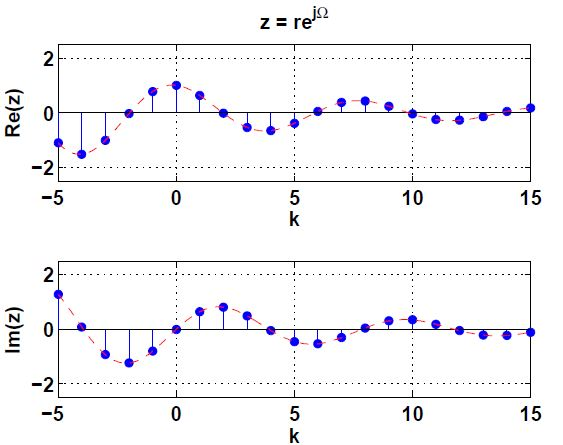
\includegraphics[scale=0.3]{Figures/z_transform/exp_signal}
\caption{Complex Exponential Discrete Signal}
\label{fig:z_transform:exp_signal}
\end{figure}


\end{itemize}

\end{frame}

\subsection{Eigenfunction Property} 
\begin{frame}[t,allowframebreaks]{Eigenfunction Property}

\begin{itemize}

\item In this part we will now why we are interested in power signal $z^k$ 

\item We will apply $z^k$ as an input to discrete linear-time invariant system

\item Computation:


$\begin{array}{rcl}
y[k] \, &=& \, h[k] \, * x[k] \\ \\
		&=& \, \displaystyle\sum_{m \, = \, - \infty}^{+ \infty} h[m] \, \times \, x[k \, - \, m] \\
		&=& \, \displaystyle\sum_{m \, = \, - \infty}^{+ \infty} h[m] \, \times \, z^{k \, - \, m} \\ \\
		&=& \, z^k \, \times \, \left(\, \displaystyle\sum_{m \, = \, - \infty}^{+ \infty} h[m] \, \times \, z^{- \, m} \, \right)\\
		&& \, \text{We pull out } z^k \text{ since the summation is a function of } m
\end{array}$

\item For a exponential input signal $z^k$, the \textcolor{red}{response} $y$ is a \textcolor{red}{scaled version} of the input signal $z^k$

\item The signal  $z^k \, = \, (r \, e^{j \, \Omega})^k$ is called \textcolor{red}{eigenfunction} because an eigenfunction applied to a system, \textcolor{red}{give output = to the input but with a scaling factor}

\end{itemize}


\end{frame}

\subsection{Transfer function}
\begin{frame}[t,allowframebreaks]{Transfer function}

\begin{itemize}

\item In the computations of the response of the complex exponential signal, the scaled version is a special quantity called \textcolor{red}{transfer function} $H(z)$ defined as:

\begin{equation}
H(z) \, = \, \displaystyle\sum_{k \, = \, - \infty}^{+ \infty} h[k] \, \times \, z^k
\end{equation}

where $h[k]$ is the impulse response of the discrete time LTI system.

\end{itemize}

\end{frame}

\subsection{Summary}
\begin{frame}[t,allowframebreaks]{Summary Eigenfunction Property}

\begin{itemize}

\item For a complex exponential signal $z^k \, = \, (r \, e^{j \, \Omega})^k$ applied as input, we get the following response

\begin{equation}
\begin{array}{rcl}
y[k] \, &=& \, z^k \, \times \, \displaystyle\sum_{m \, = \, - \infty}^{+ \infty} h[m] \, \times \, z^m \\ \\
&=& \, H(z) \, \times \, z^k  
\end{array}
\end{equation}

	\begin{itemize}
	\item $z^k$ \textcolor{red}{eigenfunction} of the system with associated eigenvalue $H(z)$ 
	\end{itemize}


\item As any complex number, $H(z) \, = \, |H(z)| \, e^{j \, \phi(z)}$, so we can further develop the response $y[k]$ as:

\begin{equation}
\begin{array}{rcl}
y[k] \, &=& \, z^k \, \times \, \displaystyle\sum_{m \, = \, - \infty}^{+ \infty} h[m] \, \times \, z^{-m} \\ \\
&=& \, H(z) \, \times \, z^k \\ \\
&=& |H(z)| \, e^{j \, \phi(z)}   \times \, z^k 
\end{array}
\end{equation}

	\begin{itemize}
	\item Interpretation: the system $H(z)$ \textcolor{red}{change only} the \textcolor{red}{amplitude} and the \textcolor{red}{phase} of the \textcolor{red}{input signal} $z^k$
	
	\item But it \textcolor{red}{won't change its frequency} $\Omega$
	\end{itemize}

\end{itemize}


\end{frame}


\subsection{Definitions}
\begin{frame}[t,allowframebreaks]{$Z$-Transform Definitions}

\begin{definition}

The \textcolor{red}{bilateral $z$-transform} of a discrete time signal $x[k]$ is:

\begin{equation}
X(z) \, = \, \displaystyle\sum_{k \, = \, - \infty}^{+ \infty} x[k] \, \times \, z^{-k} 
\end{equation}

\end{definition}

\begin{definition}

The \textcolor{red}{inverse bilateral z-transform} of a $X[z]$ is:

\begin{equation}
x[k] \, = \, \displaystyle\frac{1}{2 \, \pi \, j} \displaystyle\oint X(z) \, z^{k \, - \, 1} \, dz
\end{equation}

\end{definition}

\newpage
\begin{itemize}

\item In most of the times we are going to use the bilateral definition of the z-transform

	\begin{itemize}
	\item But also we will use the \textcolor{red}{unilateral} definition for \textcolor{red}{causal signals}
	
	\item Make life easier when dealing with region of convergence issues
	\end{itemize}

\item We won't apply complex contour integral to compute the inverse z-transform

	\begin{itemize}
	\item Instead, we will deal with simpler methods 
	\end{itemize}

\end{itemize}

\end{frame}

\subsection{Convergence}
\begin{frame}[t,allowframebreaks]{Convergence}

\begin{itemize}

\item The $z$-transform definition involves infinite summation

	\begin{itemize}
	\item Whenever we do an infinite sum, we ask the question  when does this sum converge ?
	\end{itemize}

\item Back to the definition of $z$-transform, the sum will converge if we have if the product $x[k] \, \times \, z^{-k}$ is \textcolor{red}{absolute summable}

\item Let's decompose $x[k] \, \times \, z^{-k}$:

	\begin{itemize}
	\item Recall that $z \, = \, r \, e^{j \, \Omega}$
	
	\item $\lvert \,x[k] \,z^{-k}  \,\rvert \, = \, \lvert \,x[k] \,r^{-k} \, e^{-k \, j \, \Omega}  \,\rvert \, = \lvert \,x[k] \,r^{-k} \,\rvert$
	\end{itemize}

\item So $z$-transform when $\displaystyle\sum_{k \, = \, - \infty}^{+ \infty} \lvert \,x[k] \,r^{-k} \,\rvert \, < \, \infty$

	\begin{itemize}
	\item Values of $r$ for which we have convergence is called \textcolor{red}{region of convergence}
	\end{itemize}

\end{itemize}


\end{frame}

\begin{frame}[t,allowframebreaks]{Convergence Example: DTFT and $Z$-transform}

\begin{itemize}

\item We take the following discrete time signal

\begin{figure}[ht]
\centering
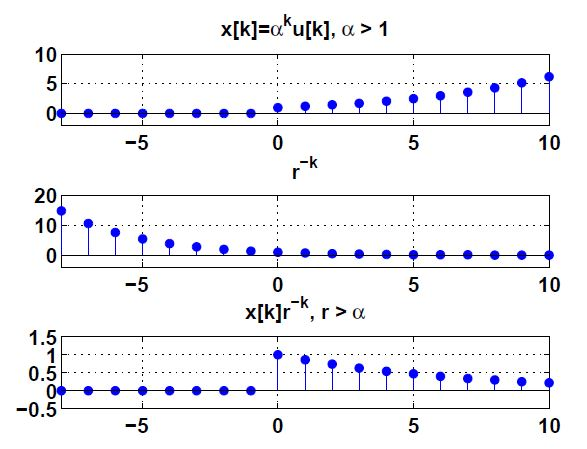
\includegraphics[scale=0.3]{Figures/z_transform/convergence_example}
\caption{DTFT of $x[k]$ doesn't exist, but z-transform exist}
\label{fig:z_transform:convergence_example}
\end{figure}

\newpage
\item $x[k]$ is increasing

	\begin{itemize}
	\item So the DTFT computation can't be done since the signal won't converge
	\end{itemize}

\item However, in Z-transform, we don't only look a the signal $x[k]$, but also with the free variable $r$

	\begin{itemize}
	\item Notice for a value $r \, > \, \alpha$, the product $x[k] \, r^{-k}$ decrease in discrete time
	\end{itemize}

\end{itemize}

\end{frame}

\begin{frame}[t,allowframebreaks]{The $Z$-Plane and DTFT}

\begin{itemize}

\item We have talked about the definition of the $z$-transform, and its convergence

\item One final point before application is the $Z$-plane

\item The $z$-plane is just a complex plane where we have the real and imaginary part of $z$ for various value of $r$ and $\Omega$


\newpage

\item A plot is shown in figure \autoref{fig:z_transform:z_plane}.

\begin{figure}[ht]
\centering
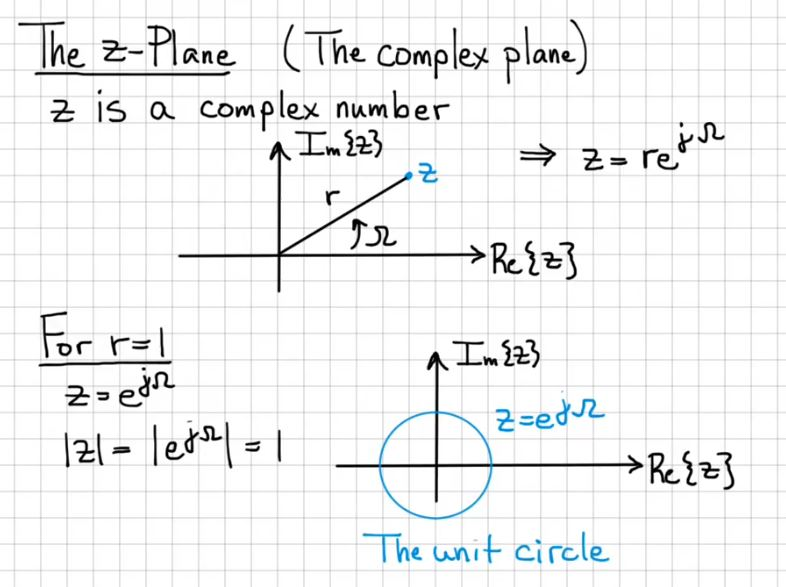
\includegraphics[scale=0.3]{Figures/z_transform/z_plane}
\caption{Z-plane Plot}
\label{fig:z_transform:z_plane}
\end{figure}

\end{itemize}

\end{frame}

\begin{frame}[t,allowframebreaks]{DTFT and Z-transform Relation}

\begin{itemize}

\item One important thing we can notice that is if set $r \, = \, 1$ and apply the definition of the $Z$-transform we get:

$\begin{array}{rcl}
X(z) \, = \, \displaystyle\sum_{k \, = \, - \infty}^{+ \infty} x[k] \, \times \, z^{-k} \, = \, \displaystyle\sum_{k \, = \, - \infty}^{+ \infty} x[k] \, \times \, r^{-k} \, e^{-j \, k \, \Omega} \, = \, \\ \displaystyle\sum_{k \, = \, - \infty}^{+ \infty} x[k] \, \times \, 1 \, \times  \, e^{-j \, k \, \Omega} \, = \,
\displaystyle\sum_{k \, = \, - \infty}^{+ \infty} x[k] \, \times \, e^{-j \, k \, \Omega}  
\end{array}$

\item So for $r \, = \, 1$, we can extract the DTFT from the $Z$-transform

	\begin{itemize}
	\item In other words, from the points on the unit circle in the $z$-plane
	\end{itemize}

\end{itemize}


\end{frame}


\subsection{Examples}

\begin{frame}[t,allowframebreaks]{Example 1: Finite Duration Discrete Time Signal}

\begin{itemize}

\item Given and Solution

\begin{figure}[ht]
\centering
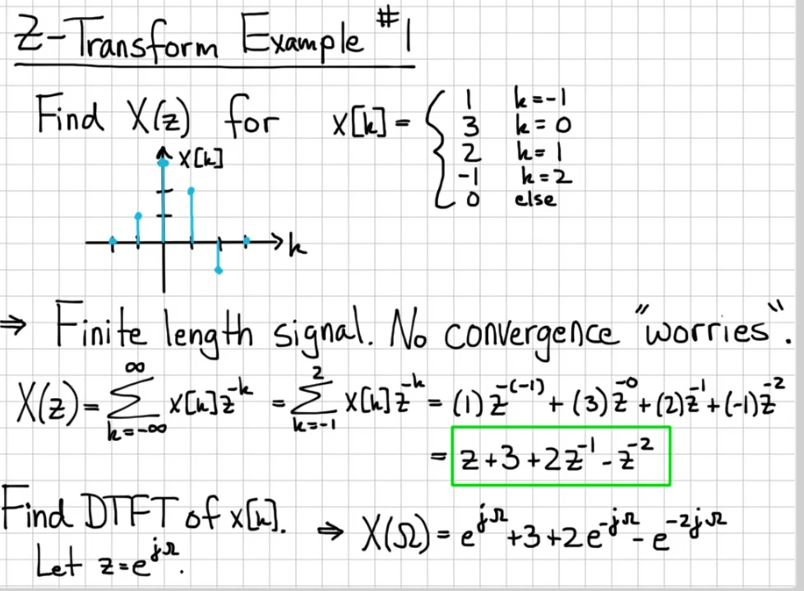
\includegraphics[scale=0.3]{Figures/z_transform/example_finite_duration}
\label{fig:z_transform:example_finite_duration}
\end{figure}

\item Since the signal is finite duration $\leftrightarrow$ no worries about convergence issues

\item We can evaluate DTFT of $x[k]$ by evaluating the z-transform at $r \, = \, 1$

\item Since the \textcolor{red}{region of convergence contains the unit circle}, we can use $z \, = \, e^{j \, \omega_d}$

\item The only points which are outside the region of convergence for a z-polynomial are 0 and $\pm \infty$

\end{itemize}


\end{frame}



\subsubsection{Finite Duration Causal Discrete Time Signal with multiples poles and zeros}
\begin{frame}[t,allowframebreaks]{Example 2: Infinite Duration Causal Discrete Time Signal}

\begin{figure}[ht]
\centering
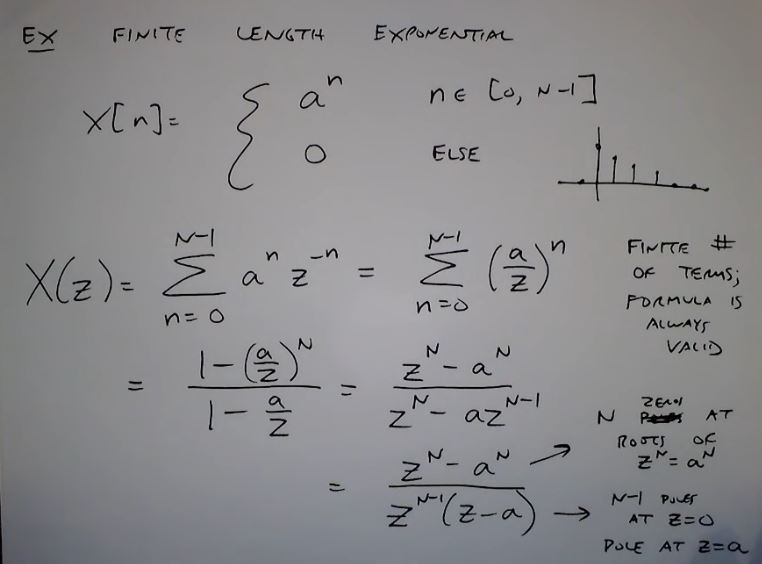
\includegraphics[scale=0.3]{Figures/z_transform/example_finite_duration_causal_many_poles_1}
\end{figure}

\newpage
\begin{figure}[ht]
\centering
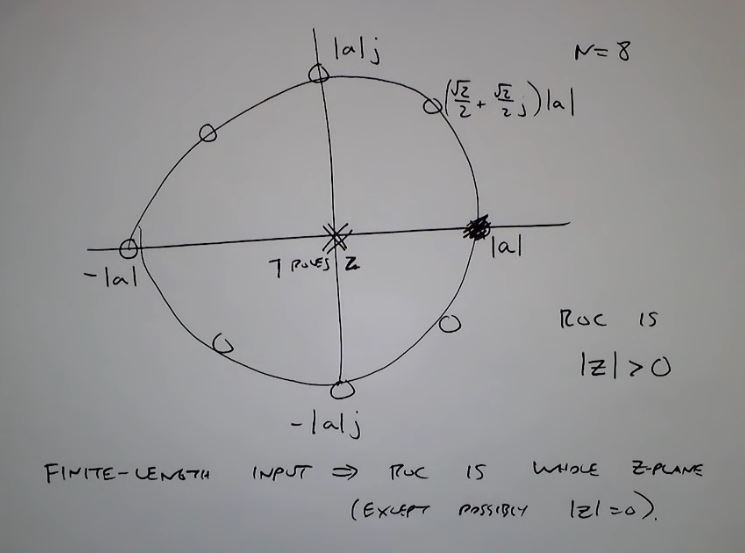
\includegraphics[scale=0.3]{Figures/z_transform/example_finite_duration_causal_many_poles_2}
\end{figure}


\end{frame}



\subsubsection{Infinite Duration Causal Discrete Time Signal}
\begin{frame}[t,allowframebreaks]{Example 2: Infinite Duration Causal Discrete Time Signal}

\begin{itemize}

\item Given and Solution

\begin{figure}[ht]
\centering
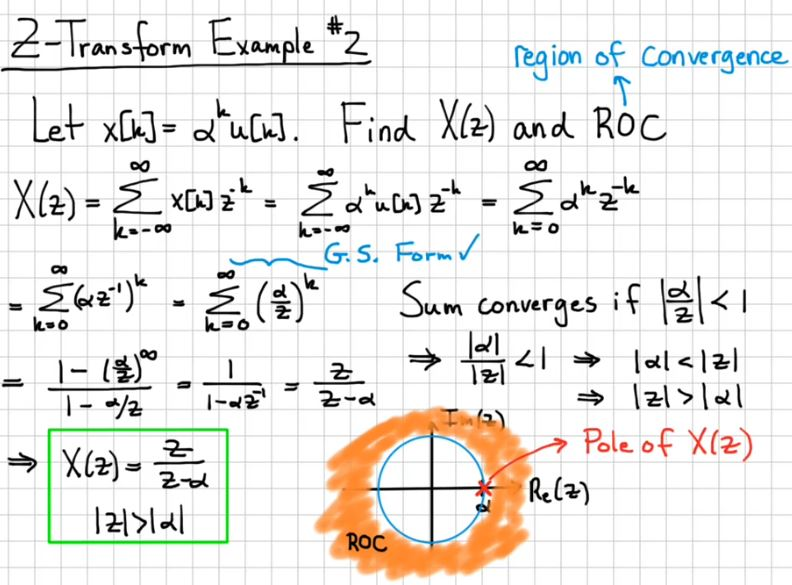
\includegraphics[scale=0.3]{Figures/z_transform/example_infinite_duration_causal_signal}
\label{fig:z_transform:example_infinite_duration_causal_signal}
\end{figure}

\newpage
\item We use the geometric series formula to evaluate the sum

\item Before directly using the geometric series formula, we need to determine the convergence since we have $\left( \, \displaystyle\frac{\alpha}{z} \, \right)^k$

\item The points outside the circle of radius $\alpha$ is the region of convergence

	\begin{itemize}
	\item For a points at $\alpha$, $X(z) \rightarrow \, \infty$
	\end{itemize}

\end{itemize}

\end{frame}


\subsubsection{Infinite Duration Anti-Causal Discrete Time Signal}
\begin{frame}[t,allowframebreaks]{Example 3: Infinite Duration Anti-Causal Discrete Time Signal}

\begin{itemize}

\item Given and Solution

\begin{figure}[ht]
\centering
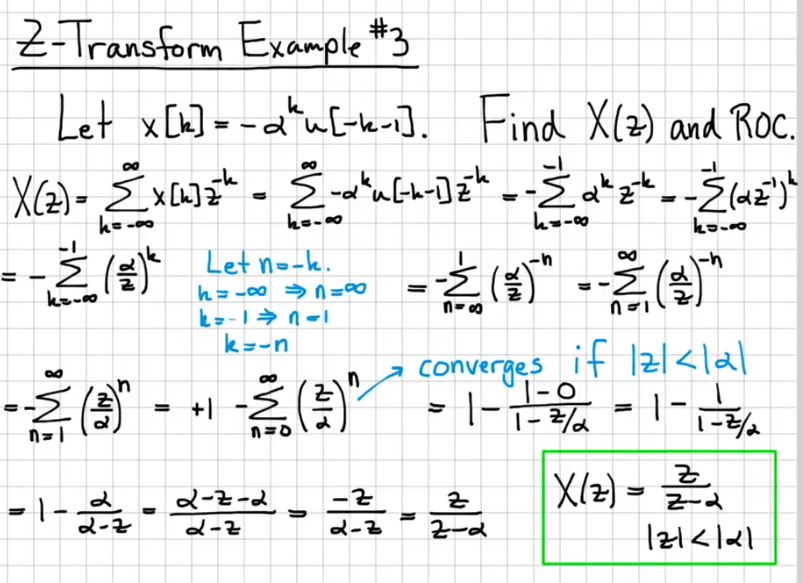
\includegraphics[scale=0.3]{Figures/z_transform/example_infinite_duration_anticausal_signal}
\label{fig:z_transform:example_infinite_duration_anticausal_signal}
\end{figure}

\item In the computation step where we have $ - \, \displaystyle\sum_{n \, = \, 1}^{\infty} \left( \, \displaystyle\frac{z}{\alpha} \, \right)^n \, = \, +1 \, - \,  \displaystyle\sum_{n \, = \, 0}^{\infty} \left( \, \displaystyle\frac{z}{\alpha} \, \right)^n $:

	\begin{itemize}
	\item We have change the summation limits from $n \, = \, 1 \rightarrow \, n \, = \, 0$, so we have add a -1 term (since we have $-$ outside), so we need to add +1 to compensate the result
	\end{itemize}

\newpage

\begin{figure}[ht]
\centering
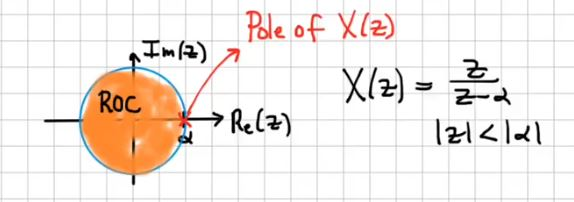
\includegraphics[scale=0.6]{Figures/z_transform/example_infinite_duration_anticausal_signal_roc}
\label{fig:z_transform:example_infinite_duration_anticausal_signal_roc}
\end{figure}

\end{itemize}

\end{frame}


\subsubsection{2 Causal Signals}
\begin{frame}[t]{2 Causal Signals}

\begin{itemize}
    \item If we have 2 signals which adds up, then the resulting ROC is the intersection of the individual ROC of each signal
    
\begin{figure}[ht]
\centering
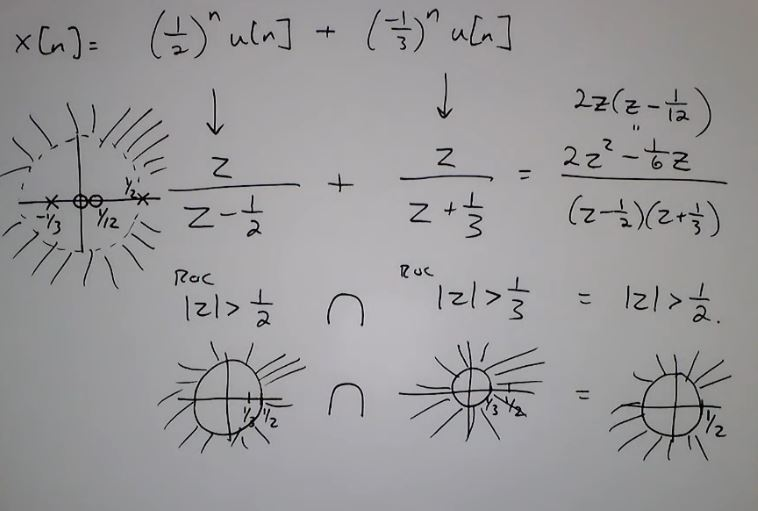
\includegraphics[scale=0.3]{Figures/z_transform/2_signals}
\label{fig:z_transform:summary_examples}
\end{figure}   
    
\item For $\lvert \, z \, \rvert \, > \, \displaystyle\frac{1}{3} \, \displaystyle \cap \, \lvert \, z \, \rvert \, > \, \displaystyle\frac{1}{2} \, \rightarrow \,  \lvert \, z \, \rvert \, > \, \displaystyle\frac{1}{2}$
    
\end{itemize}

\end{frame}


\subsubsection{Causal and Anticausal Signals}
\begin{frame}[t]{Causal and Anticausal Signals}

\begin{itemize}
    \item Now we take \textcolor{red}{causal and anticausal signals} $\leftrightarrow$ this give rise to a \textcolor{red}{double-sided signal} 
    
\begin{figure}[ht]
\centering
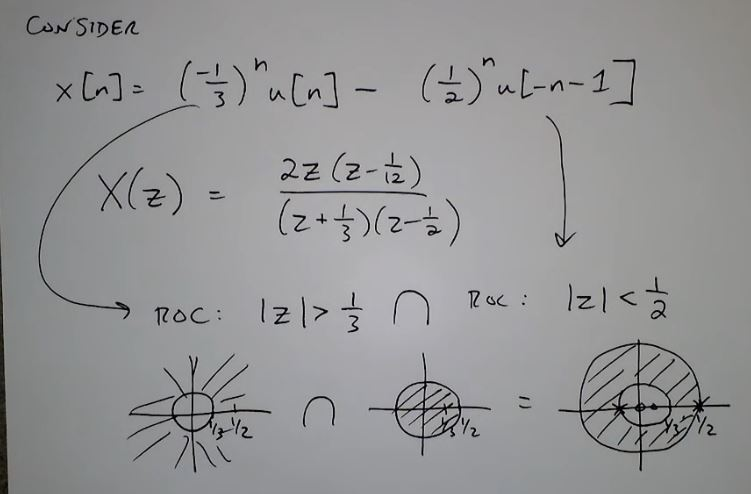
\includegraphics[scale=0.3]{Figures/z_transform/2_signals_b}
\label{fig:z_transform:summary_examples}
\end{figure}   
    
\item Notice that they have same $z$-transform, but different ROC region    
    
    
\end{itemize}

\end{frame}



\subsubsection{Summary Examples}
\begin{frame}[t,allowframebreaks]{Summary on Examples for Computing $Z$-Transform}

\begin{itemize}


\item Always Recall the rule: when using $X(z)$, we must \textcolor{red}{specify the region of convergence} for \textcolor{red}{unique correspondence} to a discrete time signal $x[k]$


\item Summary of Examples and their different region of convergence

\begin{figure}[ht]
\centering
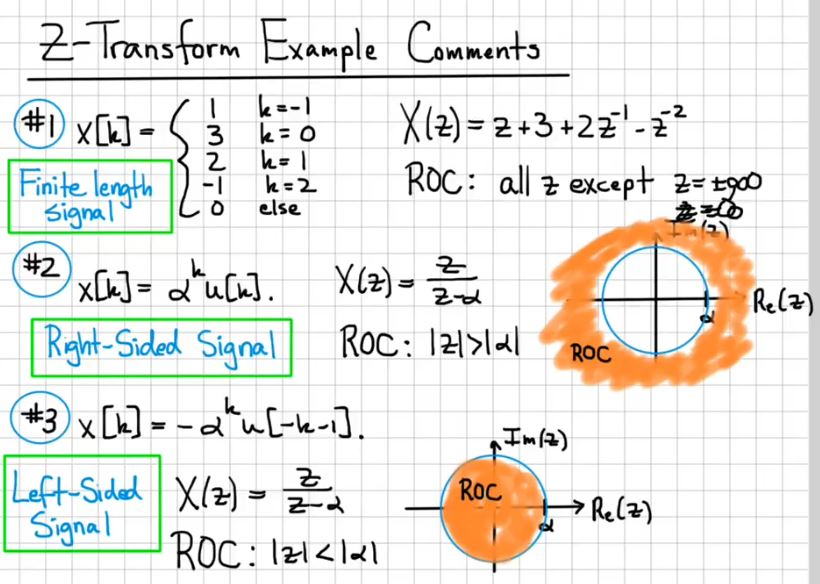
\includegraphics[scale=0.3]{Figures/z_transform/summary_examples}
\label{fig:z_transform:summary_examples}
\end{figure}

\newpage
\item Different Type of discrete time signal and their correspondent ROC

	\begin{enumerate}
	\item Finite duration  $\leftrightarrow$ all the z-plane except for 0 and $\pm \infty$
	
	\item Right sided signal $\leftrightarrow$ outside the circle
	
	\item Left sided signal $\leftrightarrow$ inside the circle
	\end{enumerate}


\item There is also 1 type of signals we didn't see: double sided signal (left and right side extension)

\item What we have done in this section is that we proved by examples different type of ROC for different type of signals

\item In the next slide, we do a general proof between ROC and the signal characteristics

\end{itemize}

\end{frame}


\subsubsection{Double Sided Signal}

\begin{frame}[t,allowframebreaks]{Double Sided Signal}

\begin{figure}[ht]
\centering
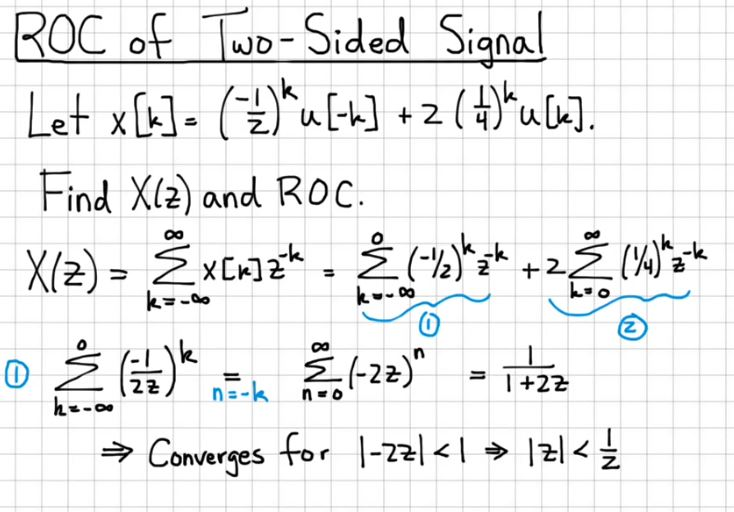
\includegraphics[scale=0.3]{Figures/z_transform/Double_Sided_negative}
\label{fig:z_transform:Double_Sided_negative}
\end{figure}

\begin{itemize}

\item We break the summation into negative part and positive part

\item In the term $\displaystyle\sum_{k \, = \, -\,\infty}^{0}$: we prefer to start the sum from 0, that's why we made the change of variable $ n \, = \, - \, k $

\end{itemize}

\newpage

\begin{figure}[ht]
\centering
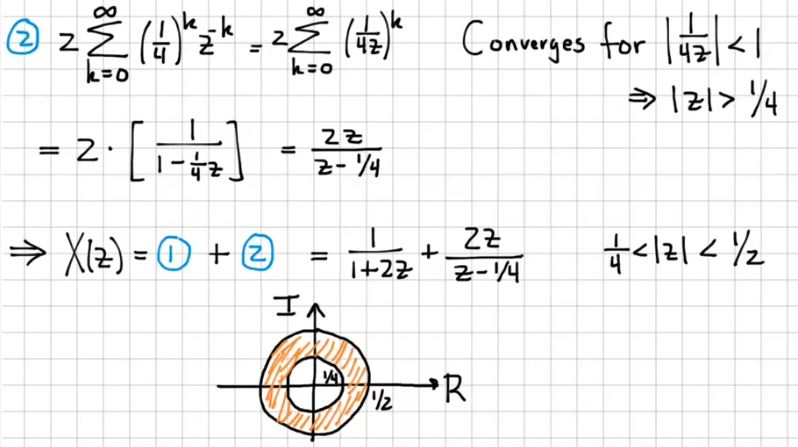
\includegraphics[scale=0.3]{Figures/z_transform/Double_Sided_positive}
\label{fig:z_transform:Double_Sided_positive}
\end{figure}

\begin{itemize}

\item We work the positive term here

\newpage
\item The ROC: it's the inequality from the negative term $\left(\,  |z| \, < \, \displaystyle\frac{1}{2}	  \,\right)$ and from the positive part $\left(\,  |z| \, > \, \displaystyle\frac{1}{4}	  \,\right)$

	\begin{itemize}
	\item This give us $ \displaystyle\frac{1}{4} < \, |z| \, < \, \displaystyle\frac{1}{2}	$
	
	\item The ROC is inside a \textcolor{red}{ring} for a \textcolor{red}{double sided discrete time signal} 
	\end{itemize}


\item Note: the circles should be plotted in dashed line and not solid, since the ROC inequality $ \displaystyle\frac{1}{4} < \, |z| \, < \, \displaystyle\frac{1}{2}	$ is \textcolor{red}{strictly less} and  \textcolor{red}{strictly above}

\end{itemize}

\end{frame}




\subsection{Theoretical Proof of Region of Convergence}
\begin{frame}[t,allowframebreaks]{Region of Convergence}

\begin{itemize}

\item To be done later


\end{itemize}


\end{frame}


\subsection{$Z$ Transform Properties}
\begin{frame}[t,allowframebreaks]{Example 1}

\begin{figure}[ht]
\centering
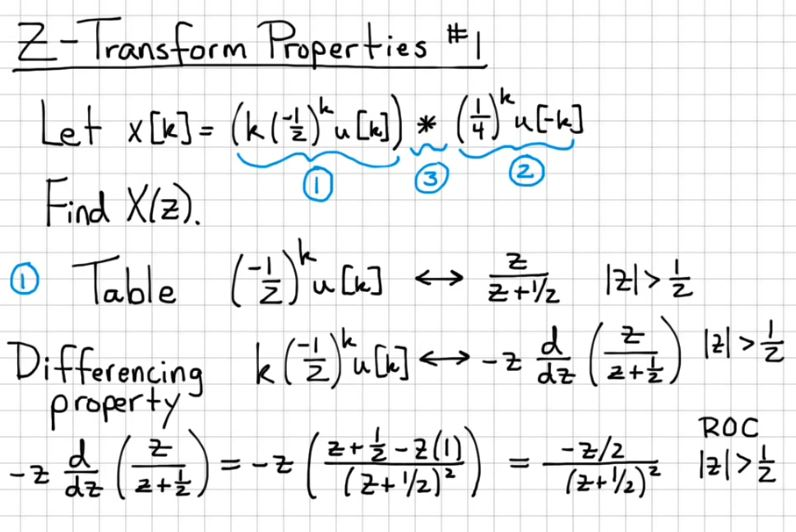
\includegraphics[scale=0.4]{Figures/z_transform/Properties_Example_1}
\label{fig:z_transform:Properties_Example_1}
\end{figure}


\begin{figure}[ht]
\centering
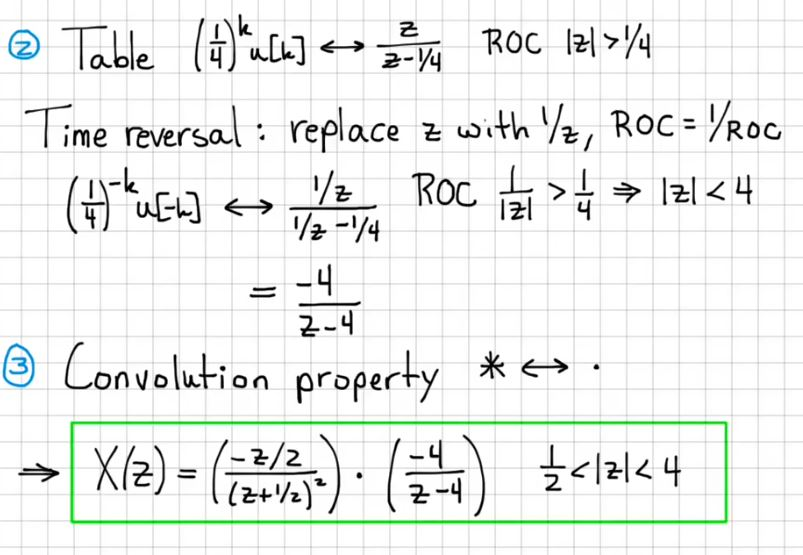
\includegraphics[scale=0.4]{Figures/z_transform/Properties_Example_1_2}
\label{fig:z_transform:Properties_Example_1_2}
\end{figure}


\end{frame}

\begin{frame}[t,allowframebreaks]{Example 2}

\begin{itemize}
\item Don't forget when using $z-$transform properties, keep track at what happen to the ROC for the final expression
\end{itemize}

\begin{figure}[ht]
\centering
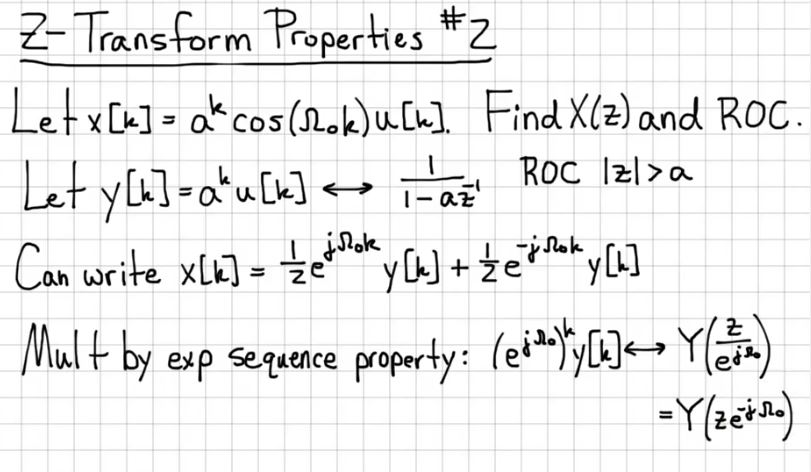
\includegraphics[scale=0.4]{Figures/z_transform/Properties_Example_2}
\label{fig:z_transform:Properties_Example_2}
\end{figure}

\begin{figure}[ht]
\centering
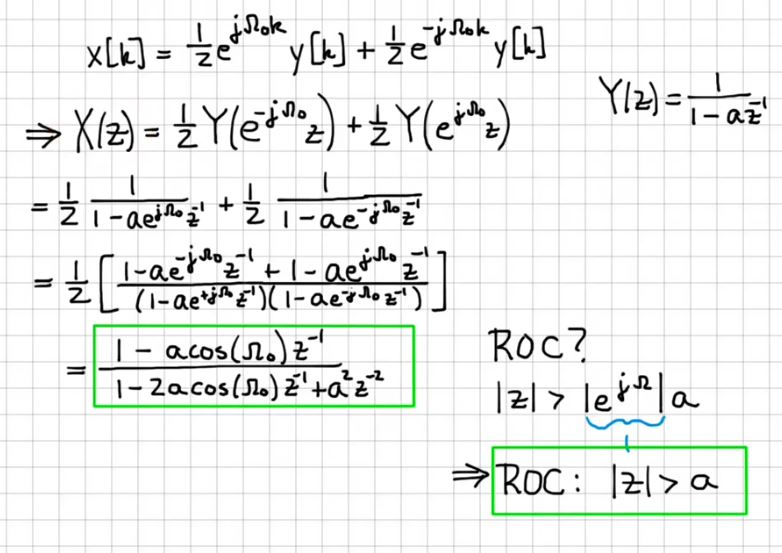
\includegraphics[scale=0.4]{Figures/z_transform/Properties_Example_2_2}
\label{fig:z_transform:Properties_Example_2_2}
\end{figure}


\end{frame}

\subsection{Pole-Zero Cancellation}

\begin{frame}[t,allowframebreaks]{Pole-Zero Cancellation}


\begin{itemize}
\item Given shown below
\end{itemize}

\begin{figure}[ht]
\centering
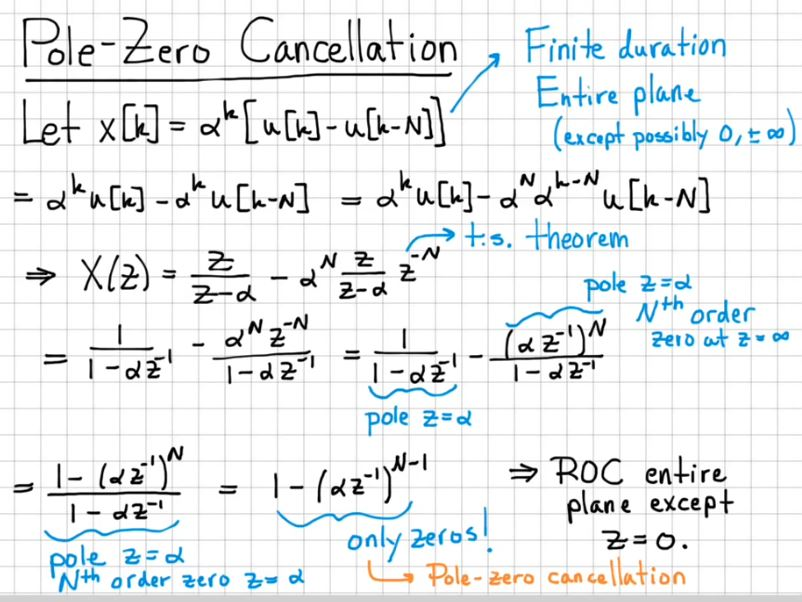
\includegraphics[scale=0.4]{Figures/z_transform/Pole_Zero_Cancellation}
\label{fig:z_transform:Pole_Zero_Cancellation}
\end{figure}

\newpage
\begin{itemize}

\item $u[k]$ turns on at $k \, = \, 0$

\item $u[k \, - \, N]$ turns on at $k \, = \, N$

\item If we subtract the 2 signals $u[k] \, - \, u[k \, - \, N]$ we get a \textcolor{red}{finite duration signal}

	\begin{itemize}
	\item \textcolor{red}{ROC} for finite duration signals is the \textcolor{red}{entire $z$ plane except for 0 and $\pm \, \infty$}
	\end{itemize}

\item $\alpha^k \ = \, \alpha^N \, \times \, \alpha^{k \, - \, N}$ so we can use the time shift theorem

\item When we have add the 2 terms $\displaystyle\frac{z}{z \, - \, \alpha}$ and $ \displaystyle\frac{z}{z \, - \, \alpha} \, z^{- \, N}$ to do simplification to the $X(z)$ expression, the zero of the numerator canceled out the pole of the denominator and we obtained finally $X(z) \, = \, 1 \, - \, \left(\, \alpha \, z^{-1} \,\right)^{N \,  - \, 1}$

	\begin{itemize}
	\item This final expression contains \textcolor{red}{only zero}
	
	\item The \textcolor{red}{ROC} has \textcolor{red}{expanded now} to contains also $\pm \, \infty$
	\end{itemize}

\item So as a conclusion, when we have some algebraic manipulation and combination of 2 expression, we may end up with an ROC bigger then what we have start in (for each expression)

\end{itemize}

\end{frame}



\subsection{Inverse $Z$-Transform}

\begin{frame}[t]{Inverse $Z$-Transform}

\begin{itemize}

\item Recall that the formal definition of the inverse of the $z$-transform:

\begin{definition}

The \textcolor{red}{inverse bilateral z-transform} of a $X[z]$ is:

\begin{equation}
x[k] \, = \, \displaystyle\frac{1}{2 \, \pi \, j} \displaystyle\oint X(z) \, z^{k \, - \, 1} \, dz
\end{equation}

\end{definition}


	\begin{itemize}
	\item We have a mathematical difficulty because we need to evaluate the \textcolor{red}{contour integral} $\displaystyle\oint$
	\end{itemize}


\item However we never use this explicit evaluation, instead we use some simpler method on practical expression of $X(z)$ encountered when dealing with discrete time LTI system:

	\begin{itemize}
	\item Ration of polynomials in function of $z^{- \, 1}$
	\end{itemize}

\end{itemize}

\end{frame}


\subsubsection{Partial Fraction Expansion (PFE)}

\begin{frame}[t]{Partial Fraction Expansion (PFE)}


\begin{itemize}

\item Ration of polynomials in function of $z^{- \, 1}$:

	\begin{equation}
	X(z) \, = \, \displaystyle\frac{B(z)}{A(z)}   \, = \, \displaystyle\frac{b_0 \, + \, b_1 \, z^{-1} \, + \, \cdots \, + \, b_M \, z^{- \, M}}{a_0 \, + \, a_1 \, z^{-1} \, + \, \cdots \, + \, a_N \, z^{- \, N}}
	\end{equation}

\item We would like to express the ration $\displaystyle\frac{B(z)}{A(z)}$ as \textcolor{red}{linear combination of $1^{\mathrm{st}}$ order terms}:

	\begin{equation}
	X(z) \, = \, \displaystyle\sum\limits_{i \, = \, 1}^N\frac{A_i}{1 \, - \, d_i \, z^{-1}}
	\label{Eq:z_transform:first_order_terms}
	\end{equation}
	
	\begin{itemize}
	\item The nice thing about equation (\autoref{Eq:z_transform:first_order_terms}) is we know their time domain expression
	\end{itemize}

\end{itemize}

\end{frame}


\begin{frame}[t]{ROC Ambiguity}

\begin{itemize}

\item However, recall that when specifying \textcolor{red}{$z$-transform}, we \textcolor{red}{always} need to \textcolor{red}{specify the ROC}

	\begin{itemize}
	\item Because 1 $X(z)$ can have several time domain expression \textcolor{red}{but always different (unique) ROC}	
	\end{itemize}

\item Concerning the $1^{\mathrm{st}}$ order $\frac{A_i}{1 \, - \, d_i \, z^{-1}}$ term, in which we have 2 choice as inverse $z$-transform:

	\begin{enumerate}
	\item $ \displaystyle\frac{A_i}{1 \, - \, d_i \, z^{-1}} A_i \, \leftrightarrow \, (d_i)^k \, \underbrace{u[k] }_{\text{right sided signal}} $ for an ROC $\underbrace{|z| \, > \, d_i}_{\text{Radius $>$ pole}}$
	
	\item  $ \displaystyle\frac{A_i}{1 \, - \, d_i \, z^{-1}} \, \leftrightarrow \, A_i \, (d_i)^k \, \underbrace{ u[\, -k \, - \, 1 \,] }_{\text{left sided signal}}\, $ for an ROC $|z| \, < \, d_i$
	\end{enumerate}

\item To \textcolor{red}{choose} the \textcolor{red}{correct discrete time domain expression}, we always need to \textcolor{red}{include} the \textcolor{red}{initial ROC of $X(z)$ before expansion}

	\begin{itemize}
	\item An example in the next slides will clear this up.
	\end{itemize}
\end{itemize}

\end{frame}


\begin{frame}[t,allowframebreaks]{Examples}

\begin{figure}[ht]
\centering
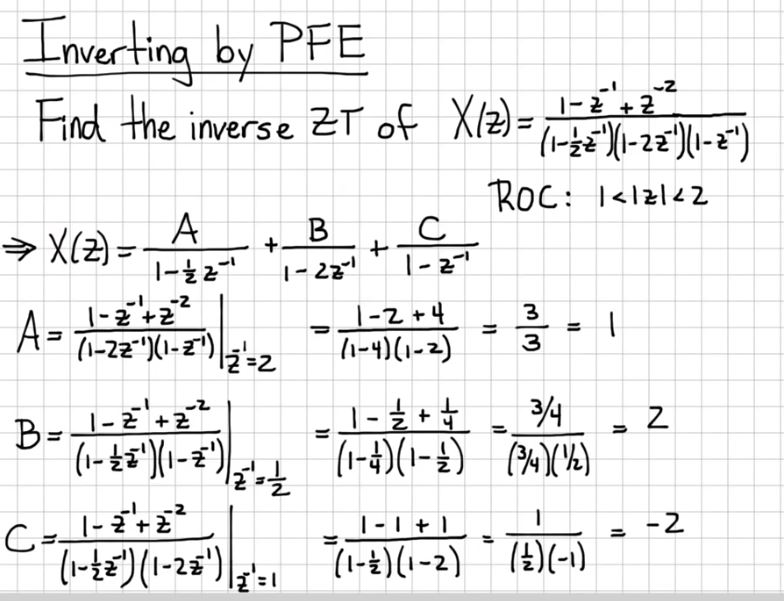
\includegraphics[scale=0.3]{Figures/z_transform/PFE_Examples_1}
\label{fig:z_transform:PFE_Examples_1}
\end{figure}

\begin{itemize}

\item The initial ROC of $X(z)$ before PFE is $ 1 \, < \, |z| \, < \, 2$

\end{itemize}

\newpage

\begin{figure}[ht]
\centering
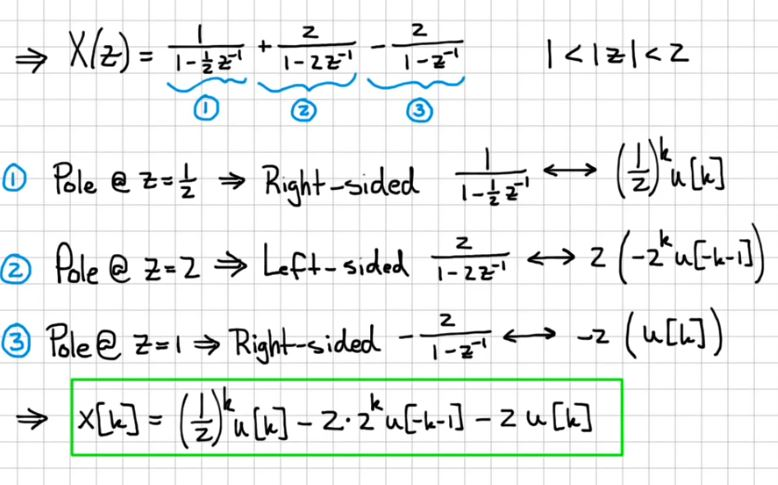
\includegraphics[scale=0.4]{Figures/z_transform/PFE_Examples_1_2}
\label{fig:z_transform:PFE_Examples_1_2}
\end{figure}

\begin{itemize}

\item Any ROC for terms 1,2 and 3 must include $ 1 \, < \, |z| \, < \, 2$

\item Work for the ROC of each term independently 

\end{itemize}



\end{frame}

\begin{frame}[t]{Unknown Initial ROC}

\begin{itemize}
\item In the previous example, we were given the ROC of $X(z)$: $ 1 \, < \, |z| \, < \, 2$
 
\item But what if we don't have it?

\item We can \textcolor{red}{use the information we know about the signals/system we have}:

	\begin{itemize}
	\item If we know we work with \textcolor{red}{stable system} $\leftrightarrow$ DTFT exist $\leftrightarrow$ \textcolor{red}{ROC} must \textcolor{red}{include the unit circle}
	
		\begin{itemize}
		\item Signals can be left side of right side
		\end{itemize}
	
	\item If we work with \textcolor{red}{causal signals}  $\leftrightarrow$ chose the \textcolor{red}{right sided inverse} for each term 
\end{itemize}	 
 
\end{itemize}


\end{frame}


\subsubsection{Long Division Inversion}

\begin{frame}[t]{Long Division Inversion}

\begin{itemize}

\item Partial fraction expansion (PFE) is one way we can do inverse $z$-transform

\item Another way we can do  inverse $z$-transform is \textcolor{red}{long division method}, which can be done when we have \textcolor{red}{1-sided signal}

	\begin{enumerate}
	\item if ROC \textcolor{red}{inside the unite circle} $\leftrightarrow \, |z| \, < \, a \leftrightarrow \, \text{right sided signal} \, \rightarrow$ we get a \textcolor{red}{sequence of positive power} of $z$ 
	
		\item if ROC \textcolor{red}{outside the unite circle} $\leftrightarrow \, |z| \, > \, a \, \leftrightarrow \, \text{left sided signal} \, \rightarrow$ we get a \textcolor{red}{sequence of negative power} of $z^{-1}$ 
	\end{enumerate}

\end{itemize}

\end{frame}

\begin{frame}[t]{Long Division Example 1: Right Sided Signal}

\begin{figure}[ht]
\centering
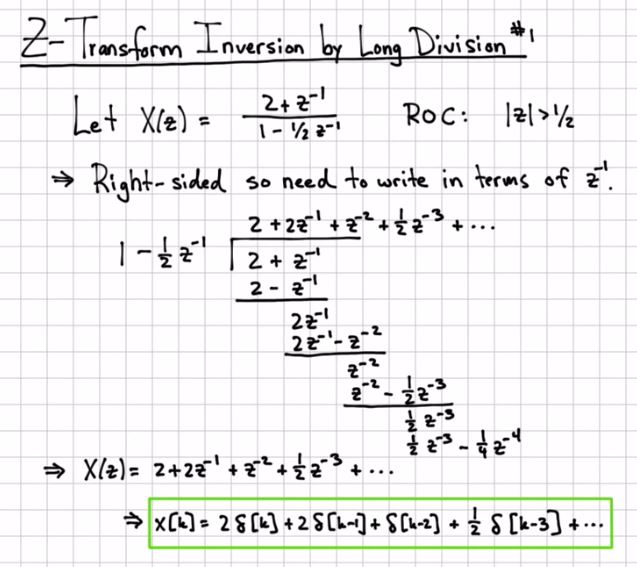
\includegraphics[scale=0.4]{Figures/z_transform/long_division_Examples_1}
\label{fig:z_transform:long_division_Examples_1}
\end{figure}

\begin{itemize}
\item $x[k]$: we have a part of the signal

\item This type of methods is useful when we need a part of the signal and not all of its components

	\begin{itemize}
	\item Example: Working with initial conditions with finite difference equations
	\end{itemize}
\end{itemize}

\end{frame}

\begin{frame}[t]{Long Division Example 2: Left Sided Signal}

\begin{figure}[ht]
\centering
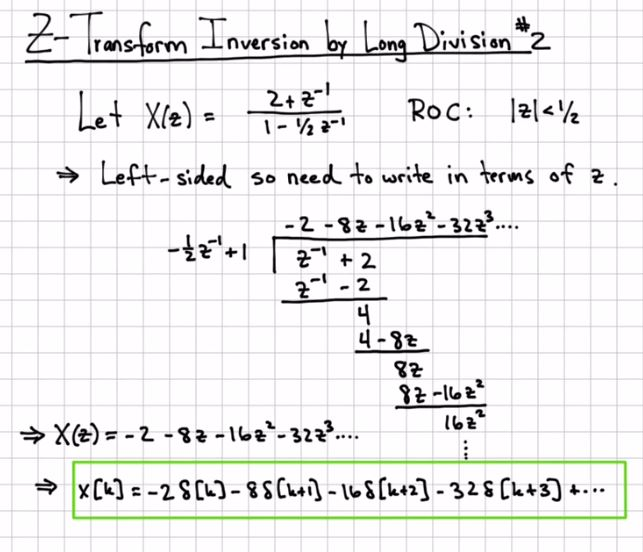
\includegraphics[scale=0.4]{Figures/z_transform/long_division_Examples_2}
\label{fig:z_transform:long_division_Examples_2}
\end{figure}


\end{frame}



\subsection{System Analysis and Transfer Function}

\begin{frame}[t]{System Analysis and Transfer Function}

\begin{block}{Transfer Function}
The input-output behavior of a discrete-time LTI system is
determined by the \textcolor{red}{system transfer function}

\begin{equation}
H(z) \, = \, \displaystyle\frac{Y(z)}{X(z)}
\end{equation}

\end{block}

\end{frame}


\subsubsection{Examples}

\begin{frame}[t,allowframebreaks]{Example of Finding $H(z)$ and $h(n)$}

\begin{figure}[ht]
\centering
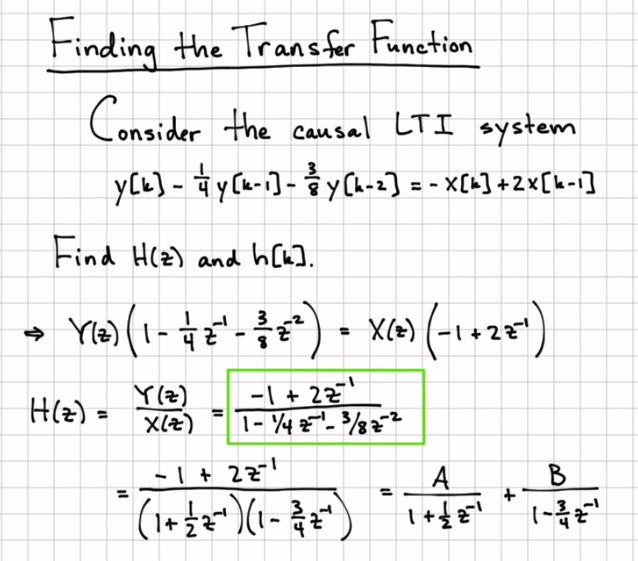
\includegraphics[scale=0.4]{Figures/z_transform/Example_transfer_function_1_1}
\label{fig:z_transform:Example_transfer_function_1_1}
\end{figure}

\newpage
\begin{figure}[ht]
\centering
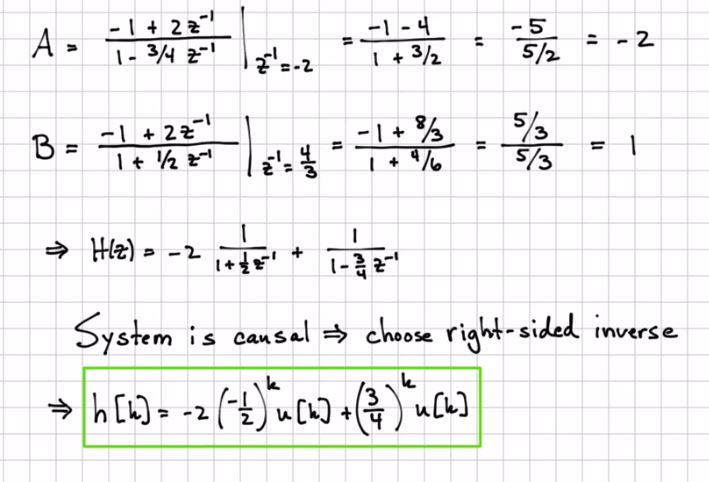
\includegraphics[scale=0.4]{Figures/z_transform/Example_transfer_function_1_2}
\label{fig:z_transform:Example_transfer_function_1_2}
\end{figure}

\end{frame}


\begin{frame}[t]{Example of Finding Difference Equation}

\begin{figure}[ht]
\centering
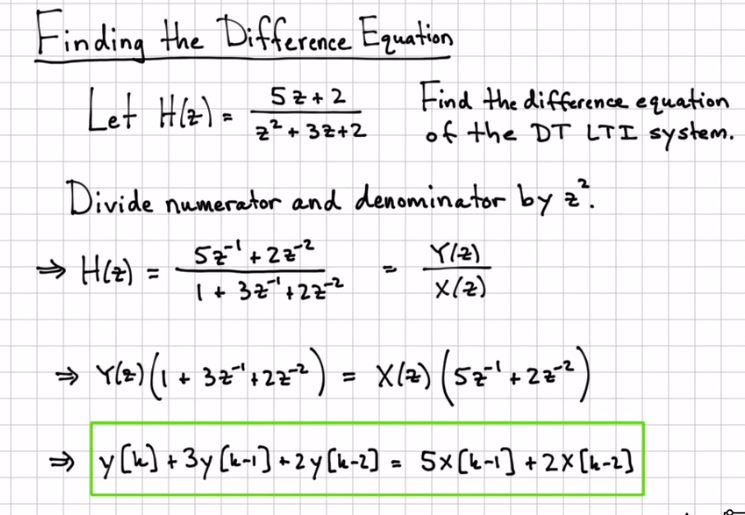
\includegraphics[scale=0.4]{Figures/z_transform/Example_Difference_Equation}
\label{fig:z_transform:Example_Difference_Equation}
\end{figure}


\end{frame}

\begin{frame}[t,allowframebreaks]{System Identification}

\begin{figure}[ht]
\centering
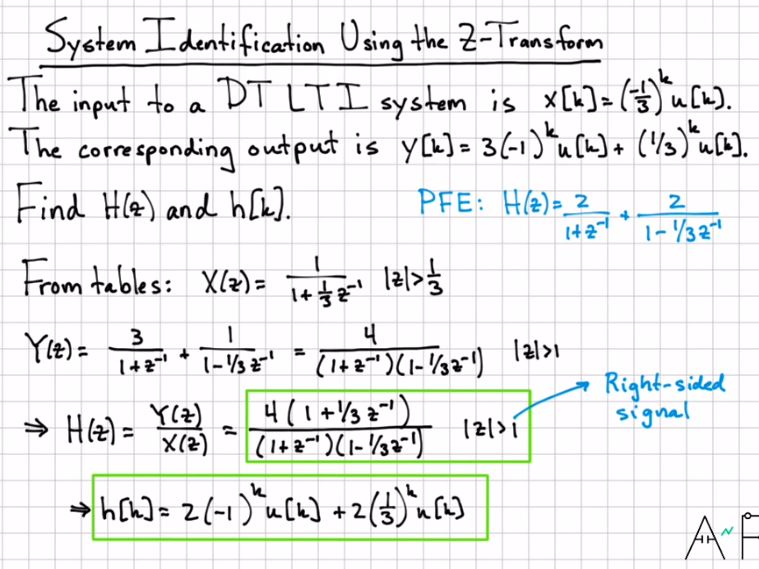
\includegraphics[scale=0.4]{Figures/z_transform/system_identification}
\label{fig:z_transform:system_identification}
\end{figure}


\begin{itemize}

\item Be aware that we need to \textcolor{red}{keep track the ROC} when computing $H(z)$ using $Y(z)$ and $X(z)$:

	\begin{itemize}
	\item $|z| \, > \, \displaystyle\frac{1}{3}$ and $|z| \, > \, 1$
	
	\item The \textcolor{red}{common area} is $|z| \, > \, 1$
	\end{itemize}

\item When solving for $h(n)$ by \textcolor{red}{taking inverse of $H(z)$}: need to be careful \textcolor{red}{which time domain signal to choose}: \textcolor{red}{right} or \textcolor{red}{left} sided

	\begin{itemize}
	\item But since ROC for $H(z)$ is $|z| \, > \, 1 \rightarrow$ we choose right sided signals
	\end{itemize}

\end{itemize}


\end{frame}


\subsubsection{Causality and Stability}

\begin{frame}[t]{Causality and Stability}

\begin{itemize}

\item In this section, we will \textcolor{red}{examine the transfer function} and try to learn what \textcolor{red}{information} we can get about the \textcolor{red}{behavior} of the \textcolor{red}{system}


\item These information will be the governed by the \textcolor{red}{location of the poles of the system}

\item Location of the pole if it is outside the unite circle, we get either:

	\begin{enumerate}
	\item A decaying exponential $\leftrightarrow$ Non-causal but stable
	
	\item An increasing right sided exponential $\leftrightarrow$ Causal but not stable	
	\end{enumerate}

\item To ensure \textcolor{red}{stability and causality}: \textcolor{red}{poles} must be \textcolor{red}{inside the unit circle}

\end{itemize}

\end{frame}



\begin{frame}[t]{Example: Find $h[k]$ for a Stable System}

\begin{figure}[ht]
\centering
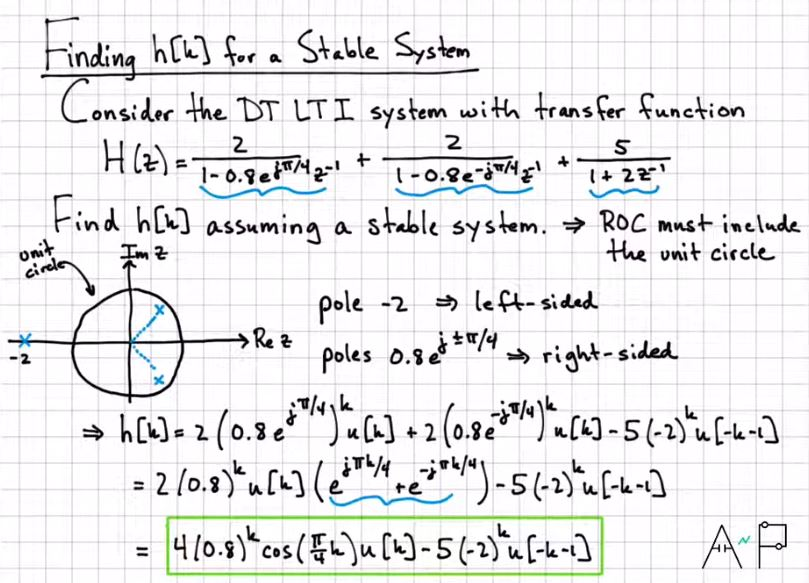
\includegraphics[scale=0.4]{Figures/z_transform/impulse_response_stable_system_example}
\label{fig:z_transform:impulse_response_stable_system_example}
\end{figure}


\end{frame}

\begin{frame}[t]{Example: Find $h[k]$ for a Stable System}

\begin{itemize}

\item Since we are assuming that the system is stable, the ROC must include the unit circle

	\begin{itemize}
	\item So we need to be aware when taking $z$-inverse for each of the term in $H(z)$ expression
	\end{itemize}

\item For the pole $= \, - \, 2$: we need to include the unit circle so we choose a left sided signal

\item The other complex poles: they are inside the unit circle, and want to include the unit circle, so we take the ROC outside and hence we need a right sided signal

\end{itemize}


\end{frame}


\begin{frame}[t]{Example: Find $h[k]$ for a Causal System}

\begin{figure}[ht]
\centering
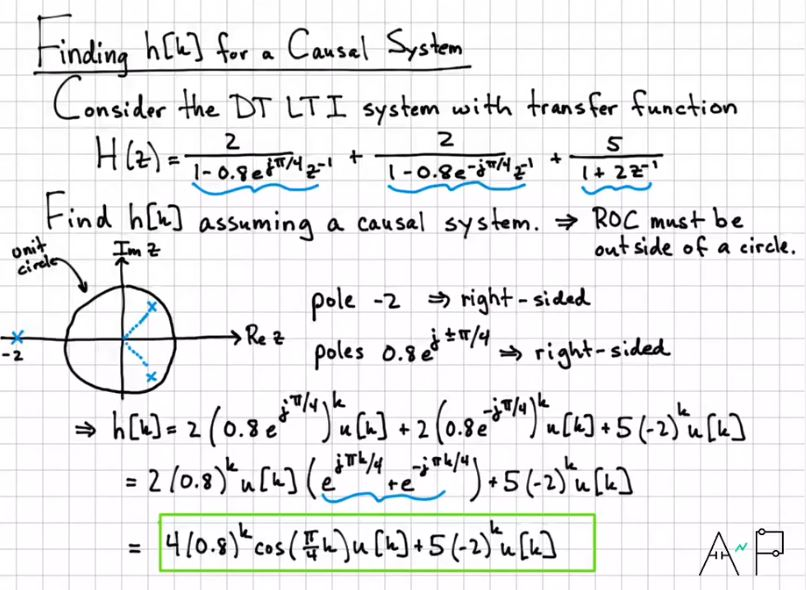
\includegraphics[scale=0.4]{Figures/z_transform/impulse_response_causal_system_example}
\label{fig:z_transform:impulse_response_causal_system_example}
\end{figure}

\end{frame}

\begin{frame}[t]{Example: Find $h[k]$ for a Causal System}

\begin{itemize}

\item For a \textcolor{red}{causal system}, things are easier

\item The \textcolor{red}{ROC} need to be \textcolor{red}{outside the unit circle}

	\begin{itemize}
	\item So for every pole we have, we choose a right sided signal 
	\end{itemize}

\end{itemize}

\end{frame}


\subsection{Inverse Linear System and Minimum Phase}

\begin{frame}[t]{Inverse Linear System and Minimum Phase}

\begin{itemize}

\item Suppose we want to compute the transfer function that \textcolor{red}{undo the effect} of our original system $h[n]$

\item By definition, such an inverse system if we convolve its impulse response $h_{\text{inv}}[n]$ with $h[n]$ we obtain a pulse $\delta[n]$

\begin{equation}
(\,h_{\text{inv}} \, \star \, h \,)[n] \, = \, \delta[n]
\end{equation}

\item Taking this definition into the $z$-domain we have:

\begin{equation}
H_{\text{inv}}(z) \, \times \, H(z) \, = \, 1 
\end{equation}

\end{itemize}

\begin{block}{Definition}
The \textcolor{red}{Inverse System Transfer Function} is the inverse the transfer function of the original system

	\begin{equation}
	H_{\text{inv}}(z) \, = \, \displaystyle\frac{1}{H(z)}
	\end{equation}
\end{block}


\end{frame}

\begin{frame}[t]{Causality and Stability Inverse Linear System and Minimum Phase}

\begin{itemize}

\item When designing real word system, we want them to be \textcolor{red}{causal} and \textcolor{red}{stable}

\item Dealing with \textcolor{red}{$H_{\text{inv}}(z)$}, they have the \textcolor{red}{flipped poles and zeros of $H(z)$}

\item So if we want $H_{\text{inv}}(z)$ to be causal and stable, the \textcolor{red}{poles} and \textcolor{red}{zeros} of $H(z)$ must be \textcolor{red}{inside the unit circle}

\end{itemize}

\begin{block}{Definition}

A system $H(z)$ having \textcolor{red}{all its poles and zeros inside the unit circle} is called a \textcolor{red}{minimum phase system}

\end{block}

\end{frame}



\begin{frame}[t]{Example}

\begin{figure}[ht]
\centering
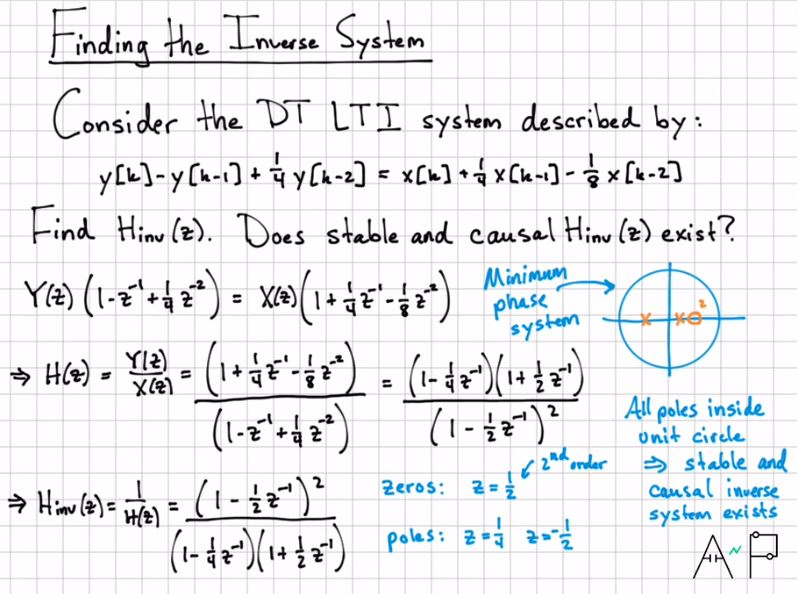
\includegraphics[scale=0.4]{Figures/z_transform/inverse_linear_sytem_example}
\label{fig:z_transform:inverse_linear_sytem_example}
\end{figure}


\end{frame}



\subsection{Frequency Response $H(\omega_d)$}

\begin{frame}[t]{Frequency Response $H(\omega_d)$ form Poles and Zeros}

\begin{itemize}

\item Now in this section we learn how to \textcolor{red}{sketch frequency response} $H(\omega_d)$ by \textcolor{red}{tracking} the \textcolor{red}{poles} and \textcolor{red}{zeros} \textcolor{red}{from the unit circle in the $z$-plane}

\item It is true that we have some programming tools that can do this for us, but be able to do this by hand will give us more understanding about the relation between the $z$-transform tools and the frequency response $H(\omega_d)$ in the DTFT domain

\end{itemize}

\end{frame}

\begin{frame}[t,allowframebreaks]{Computation}

\begin{itemize}

\item We know that we can obtain DTFT expression by letting $z \, = \, e^{j \, \omega_d}$

\item $H(z)$ is the product of zeros over the product of poles

\begin{equation}
H(z) \, = \, \displaystyle\frac{( \, z \, - \, z_1 \,) \, \times \, ( \, z \, - \, z_2 \,) \, \times \, \cdots \, \times \, ( \, z \, - \, z_n \,)}{( \, z \, - \, p_1 \,) \, \times \,( \, z \, - \, p_2 \,) \, \times \, \cdots \, \times \,( \, z \, - \, p_n \,)}
\end{equation} 

\item We let $z \, = \,  e^{j \, \omega_d}$ and make the substitution in $H(z)$:

\begin{equation}
H(\omega_d) \, = \, \displaystyle\frac{( \,  e^{j \, \omega_d} \, - \, z_1 \,) \, \times \, ( \,  e^{j \, \omega_d} \, - \, z_2 \,) \, \times \, \cdots \, \times \, ( \,  e^{j \, \omega_d} \, - \, z_n \,)}{( \,  e^{j \, \omega_d} \, - \, p_1 \,) \, \times \,( \,  e^{j \, \omega_d} \, - \, p_2 \,) \, \times \, \cdots \, \times \,( \,  e^{j \, \omega_d} \, - \, p_n \,)}
\label{Eq:z_transfomr:freq_response_2}
\end{equation} 

\newpage

\item 3 quantities are the key in equation \autoref{Eq:z_transfomr:freq_response_2}:

	\begin{enumerate}
	\item The quantity $e^{j \, \omega_d}$ is on the unit circle
	
	\item The quantity $ e^{j \, \omega_d} \, - \, z_i$ is a vector from $z_i \, \rightarrow \, e^{j \, \omega_d}$
	
	
	\item The quantity $ e^{j \, \omega_d} \, - \, p_i$ is a vector from $p_i \, \rightarrow \, e^{j \, \omega_d}$
	\end{enumerate}


\item So we can write these vectors using polar expression as:

\begin{equation}
\begin{array}{rcl}
r_i \, e^{j \, \phi_i} \, = \, e^{j \, \omega_d} \, - \, z_i \\
d_i \, e^{j \, \theta_i} \, =  e^{j \, \omega_d} \, - \, p_i 
\end{array}
\label{Eq:z_transfomr:freq_response_3}
\end{equation}

\item Putting equation (\autoref{Eq:z_transfomr:freq_response_3}) in equation (\autoref{Eq:z_transfomr:freq_response_2})

\begin{equation}
\begin{array}{rcl}
H(\omega_d) \, &=& \, \displaystyle\frac{( \, r_i \, e^{j \, \phi_1} \,) \, \times \, ( \,  r_i \, e^{j \, \phi_2}\,) \, \times \, \cdots \, \times \, ( \, r_i \, e^{j \, \phi_n} \,)}{( \,  d_i \, e^{j \, \theta_1} \,) \, \times \,( \, d_i \, e^{j \, \theta_2} \,) \, \times \, \cdots \, \times \,( \,  d_i \, e^{j \, \theta_n} \,)} \\ \\
		&=& \, \displaystyle\frac{r_1 \, r_2 \, \cdots \, r_n}{d_1 \, d_2 \, \cdots \, d_n} \, \times \,  \\
		&&  \text{exp} \, (\, j \, \left[ \,  ( \phi_1 \, + \, \phi_2 \, \cdots \, \phi_n ) \, - \, (\, \theta_1 \, + \, \theta_2 \, + \, \cdots \, + \, \theta_n \,) \,\right] )
\end{array}
\end{equation}

\end{itemize}


\end{frame}

\begin{frame}[t]{Formula for Amplitude and Phase Response}

\begin{equation}
\begin{array}{rcl}
\lvert\, H(\omega_d) \, \rvert \, &=& \, \displaystyle\frac{r_1 \, r_2 \, \cdots \, r_n}{d_1 \, d_2 \, \cdots \, d_n} \\ \\
 \phase{H(\omega_d)} \, &=& \, (\, \phi_1 \, + \, \phi_2 \, \cdots \, \phi_n ) \, - \, (\, \theta_1 \, + \, \theta_2 \, + \, \cdots \, + \, \theta_n \,) \\
 		&=& \text{Sum of zeros angles to } e^{j \omega_d} \, - \,  \text{Sum of poles angles to } e^{j \omega_d}
\end{array}
\end{equation}

\end{frame}


\begin{frame}[t]{Example}

\begin{figure}[ht]
\centering
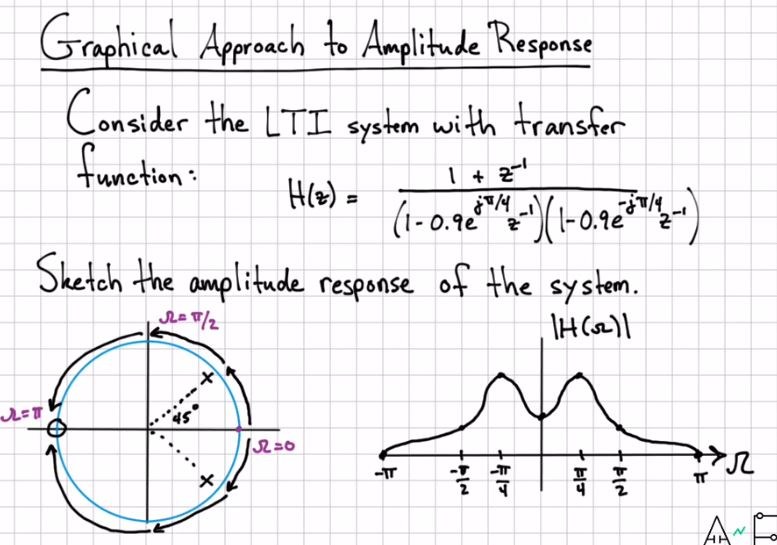
\includegraphics[scale=0.4]{Figures/z_transform/frequency_response_approximate_sketch_example}
\label{fig:z_transform:frequency_response_approximate_sketch_example}
\end{figure}


\end{frame}



\subsection{Unilateral $Z$-Transform}

\begin{frame}[t]{Introduction}

\begin{itemize}

\item Unilateral $Z$-Transform are useful if we want to \textcolor{red}{restrict} ourselves to be working with \textcolor{red}{causal signals/systems}

\item Advantage:

	\begin{itemize}
	\item Don't need to worry about the ROC $\leftrightarrow$ since the \textcolor{red}{signals} are \textcolor{red}{causal}, we know that the \textcolor{red}{ROC} will be \textcolor{red}{something outside the unite circle}
	
	\item Help us solved difference equation
	\end{itemize}



\begin{block}{Definition}

The \textcolor{red}{Unilateral $Z$-Transform} of the discrete time signal $x[k]$ is:

\begin{equation}
X(z) \, = \, \displaystyle\sum_{k \, = \, 0}^{+ \, \infty} x[k] \, z^{-k}
\end{equation}

\end{block}


\end{itemize}

\end{frame}


\subsubsection{Time Shift Properties}

\begin{frame}[t]{Time Shift Properties}

\begin{itemize}

\item All the properties of the bilateral $Z$-transform are the same for the unilateral $Z$-transform except when doing time shift

\item 2 types of time shift can be done for $N \, > \, 0 \in \, \mathbb{N}$:

	\begin{enumerate}
	\item Delay $\leftrightarrow$ shifting to the right $\leftrightarrow \, x[k \,-\, N] \, u[k]$ 
	
	\item Time Advance $\leftrightarrow$ shifting to the left $\leftrightarrow \, x[k \,+\, N] \, u[k]$ 
	\end{enumerate}

\item When plug in the 2 time shifted signal into the unilateral $Z$-transform definition we get:

\begin{equation}
\begin{array}{rcl}
x[k \,-\, N] \, u[k] \, &\leftrightarrow& \, z^{-N} \, X(z) \, + \, z^{-N} \,   \displaystyle\sum_{k \, = \, 1}^{N} x[\, -\,k \,] \, z^k  \\ \\
x[k \,+ \, N] \, u[k] \, &\leftrightarrow& \, z^N \, X(z) \, - \, z^N \,   \displaystyle\sum_{k \, = \, 0}^{N \ - \, 1} x[k] \, z^{-k}
\end{array}
\end{equation} 

\end{itemize}

\end{frame}

\begin{frame}[t]{Time Delay Pattern}

\begin{itemize}

\item $N \, = \, 1$

\begin{equation*}
x[k \, - \, 1] \, u[k] \,\leftrightarrow \,  z^{-1} \, X(z) \, + \, x[-1]
\end{equation*}

\item $N \, = \, 2$

\begin{equation*}
x[k \, - \, 2] \, u[k] \,\leftrightarrow \,  z^{-2} \, X(z)\, + \, z^{-1} \, x[-1] \, + \, x[-2]
\end{equation*}


\item $N \, = \, 3$

\begin{equation*}
x[k \, - \, 1] \, u[k] \,\leftrightarrow \,  z^{-3} \, X(z)\, + \, z^{-2} \, x[-1] \, + \, z^{-1}\, x[-2] \, + \, x[-3]
\end{equation*}

\end{itemize}

\end{frame}

\begin{frame}[t]{Observation in Time Delay Pattern}

\begin{itemize}

\item Notice that in each term for any $N$ value, the sum in each term is equal to $N$

\item Example for $N \, = \, 2$

	\begin{itemize}
	\item \begin{equation*}
x[k \, - \, 2] \, u[k] \,\leftrightarrow \,  z^{-2} \, X(z)\, + \, z^{-1} \, x[-1] \, + \, x[-2]
\end{equation*}

	\item The term $z^{-1} \, x[-1] $: we have 1 and 1 give 2
	\end{itemize}

\item Same for the terms in case of $N \, = \, 3$

	\begin{itemize}
	\item $z^{-1} \, x[-2] $: 1 and 2 give 3
	
	\item $z^{-2} \, x[-1] $: 2 and 1 give 3
	\end{itemize}

\item Same concept exist in time advance pattern

\end{itemize}

\end{frame}

\begin{frame}[t]{Time Advance Pattern}

\begin{itemize}

\item $N \, = \, 1$

\begin{equation*}
x[k \, + \, 1] \, u[k] \,\leftrightarrow \,  z \, X(z) \, - \, z \, x[0]
\end{equation*}

\item $N \, = \, 2$

\begin{equation*}
x[k \, + \, 2] \, u[k] \,\leftrightarrow \,  z^{2} \, X(z)\, - \, z^{2} \, x[0] \, - \,z \, x[	1]
\end{equation*}


\item $N \, = \, 3$

\begin{equation*}
x[k \, + \, 3] \, u[k] \,\leftrightarrow \,  z^{3} \, X(z)\, - \, z^{3} \, x[0] \, - \, z^{2}\, x[1] \, - \, z\, x[2]
\end{equation*}

\end{itemize}

\end{frame}
